\chapter{Análise Bibliográfica sobre Raytracing, por Ualiton Ventura da Silva\label{chap:bibliometria:uventura}}

\section{Planejamento do estudo}

A computação gráfica trata-se de uma área que muito desenvolveu-se nos últimos anos, principalmente devido à evolução dos processadores e a alta demanda, sendo responsável por permitir a elaboração de jogos digitais por exemplo.

Atualmente, um dos campos estudados na área trata-se de ray tracing, que utiliza uma abordagem alternativa para a renderização de imagens digitais (podendo ser utilizada em outros campos e de outras maneiras), possibilitando muitas vezes maior “realismo” no resultado gráfico final, sendo este um comportamento muito atrativo para o público mais geral em jogos, filmes ou desenhos. Contudo, deve-se ater ao fato que este “realismo” possui um custo, sendo o processamento o maior deles, anteriormente não utilizava-se esta técnica justamente por não haver processadores capazes de gerar resultados com muita facilidade ou em tempo hábil.

O estudo do presente texto busca então entender:
\begin{itemize}
    \item O crescimento da produção científica em relação ao tema
    \item Análise e desenvolvimento das fontes mais relevantes sobre o tema
    \item Artigos que foram mais relevantes
\end{itemize}

\section{Uso do Bibliometrix e Biblioshiny}

Para a realização dos estudos acerca da bibliografia, utilizou-se a ferramenta Bibliometrix e o ambiente de desenvolvimento RStudio para execução da mesma.

\section{Coleta de Dados}

A coleta de dados foi feita utilizando o site Web of Science, no dia 12 de fevereiro de 2022, sendo que seu acesso pode ser disponibilizado através do Periódicos CAPES, sendo permitido para alunos da Universidade de Brasília, dentre outras.

\subsection{Query de Busca}

Por tratar-se de um assunto específico utilizou-se apenas duas tags, sendo a query resultante:

“ray tracing and computer graphics”

Sendo “ray tracing” o abordado e “computer graphics” o domínio onde encontra-se. Buscou-se poucos termos por ser um campo recente e ainda estar em desenvolvimento. O site “Web of Science” possibilita uma filtragem das edições analisadas, contudo, manteve-se todas para ter uma análise mais completa do assunto.

\section{Análise dos Dados}

\subsection{Filtragem de Dados}

Como resultado obtiveram-se 1153 resultados, utilizou-se 1000 destes. Ao enviar os dados obtidos para a plataforma Biblioshiny uma nova filtragem foi aplicada, buscando-se somente artigos publicados (ARTICLE). Assim, 441 documentos puderam ser utilizados de 1984 a 2022.

\subsection{Análise Descritiva do Dataset}

\begin{description}
    \item[Timespan] Os artigos publicados estão entre 1984 e 2022.
    \item[Sources (Journals, Books, etc)] Das fontes dispostas são 125.
    \item[Documents] O número de artigos gerados foram 441.
    \item[Average years from publication] A média de tempo de publicação é de 13 anos.
    \item[Average citations per documents] A média de citações por documento é de 13.26.
    \item[Average citations per year per doc] A média de citação por documento em um ano é de  0.9167.
    \item[References] O número de referências utilizadas são de 9491.
    \item[Keywords Plus (ID)] O número de palavras chaves distintas são de 373.
    \item[Author's Keywords (DE)] O número de palavras chaves distintas utilizadas pelos autores é de  1061.
    \item[Authors] O número de autores obtidos foi de 1158.
    \item[Author Appearances] O número de autores existentes nas publicações é de 1451.
    \item[Single-authored documents] Os artigos publicados com somente um autor são 47.
    \item[Documents per Author] O número médio de documentos publicados por os autores é de 0.381.
    \item[Authors per Document] O número médio de autores por documentos é 2.63.
    \item[Co-Authors per Documents] Por cada documento publicado, em média existem  3.29 co-autores.
    \item[Collaboration Index] Seu índice de colaboração é 2.82.
\end{description}

\subsection{Evolução da Produção Científica}

\begin{figure}[H]
    \centering
    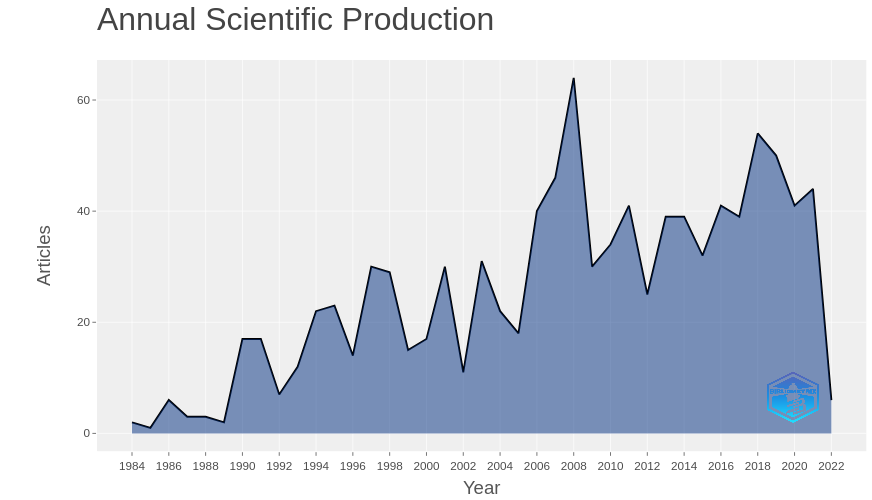
\includegraphics[width=1\textwidth]{experiments/uventura/AnaliseBibliometrica/Images/publicação-anual.png}
    \caption{Publicação Anual}
    \label{fig:uventura:bib-anual-pub}
\end{figure}

Havendo uma média de crescimento de 2.93\% ao ano, sendo compreensível o aumento anual, considerando o aumento de demanda e processamento. Mas é necessário atentar-se ao fato de que ocorrem grandes variações ao longo do tempo em relação a sua produção.

\subsection{Evolução das Citações}

Após verificar-se o crescimento da produção científica verifica-se que em relação às citações dos documentos, obtém-se graficamente que:

\begin{figure}[H]
    \centering
    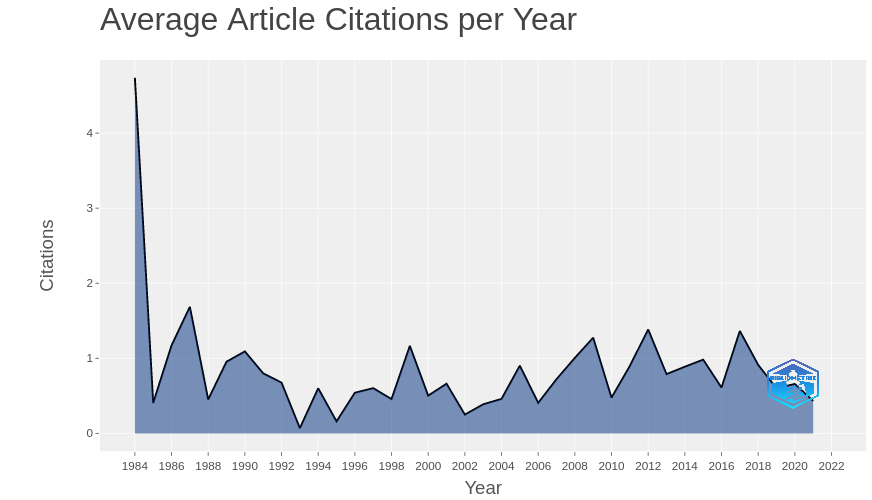
\includegraphics[width=1\textwidth]{experiments/uventura/AnaliseBibliometrica/Images/citação-anual.png}
    \caption{Citação Anual}
    \label{fig:uventura:bib-anual-cit}
\end{figure}

\subsection{Evolução das Citações}

Observa-se que apesar do crescimento em relação aos artigos publicados, é possível notar uma certa constância nas citações, ou seja, as fontes não estão constantemente em crescimento e permanecem em uma área média abaixo de 2 citações. Podem existir diversos motivos que caracterizam tal fato, um deles a ser mencionado é o próprio uso das pesquisas na área, que embora possam ter relevância, são utilizadas em meios de aplicação.

\subsection{Three-Field Plot (Sankey Diagram)}

Buscando entender então os autores do assuntos, gerou-se uma plotagem de três campos, que relaciona autores, citações frequentes e as palavras chaves por assunto, obtendo então:

\begin{figure}[H]
    \centering
    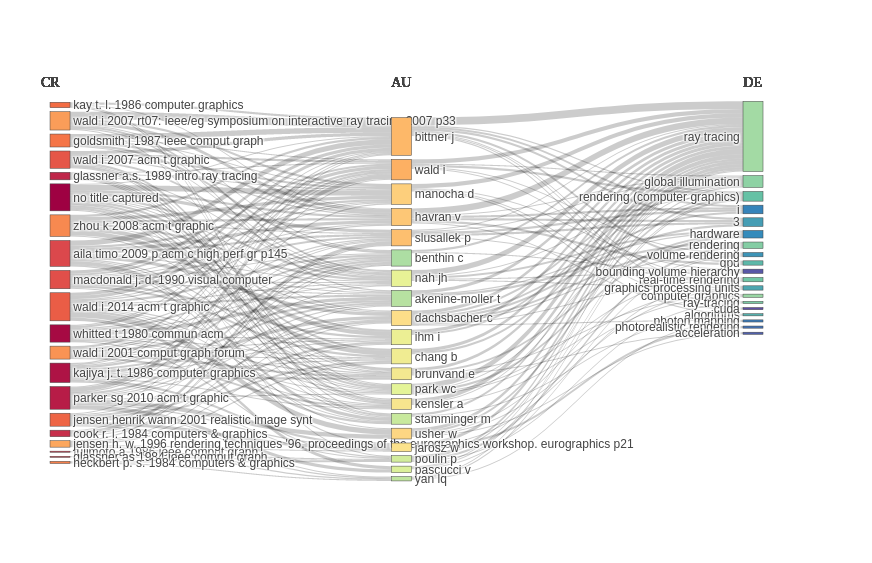
\includegraphics[width=1\textwidth]{experiments/uventura/AnaliseBibliometrica/Images/ThreeFields.png}
    \caption{Sankey Diagram}
    \label{fig:uventura:bib-three-fields}
\end{figure}

Observe que dentre os campos estudados, parte deles são, global ilumination(iluminação global), rendering (renderização), hardware, volume rendering (renderização de volume), gpu (Unidade Gráfica de Processamento), bounding volume hierarchy (hierarquia de volume delimitadora), photorealistc rendering (renderização fotorealística).

Todos os campos citados possuem enorme relevância na área, mas vamos nos ater momentaneamente a uma área para compreender o impacto dos temas tratados e a importância.

Um dos campos descritos trata-se da iluminação global, sendo esta responsável por criar efeito mais realístico de iluminação. Anteriormente a forma de iluminação de um ambiente gráfico consistia em criar uma fonte de luz que iluminava todo o ambiente, caso não fosse suficiente, acrescentariam-se outras fontes, observe que este método não descreve adequadamente a própria realidade, já que ao iluminar um objeto este objeto irá refletir a luz que então alcançará outras superfícies, é esta característica que permite ambientes mais “vívidos” na composição de luz. Abaixo seguem exemplos sem iluminação global e com iluminação global respectivamente, observe como sem seu uso o resultado final é uma imagem mais escura e que não penetra as superfícies.

\begin{figure}[H]
    \centering
    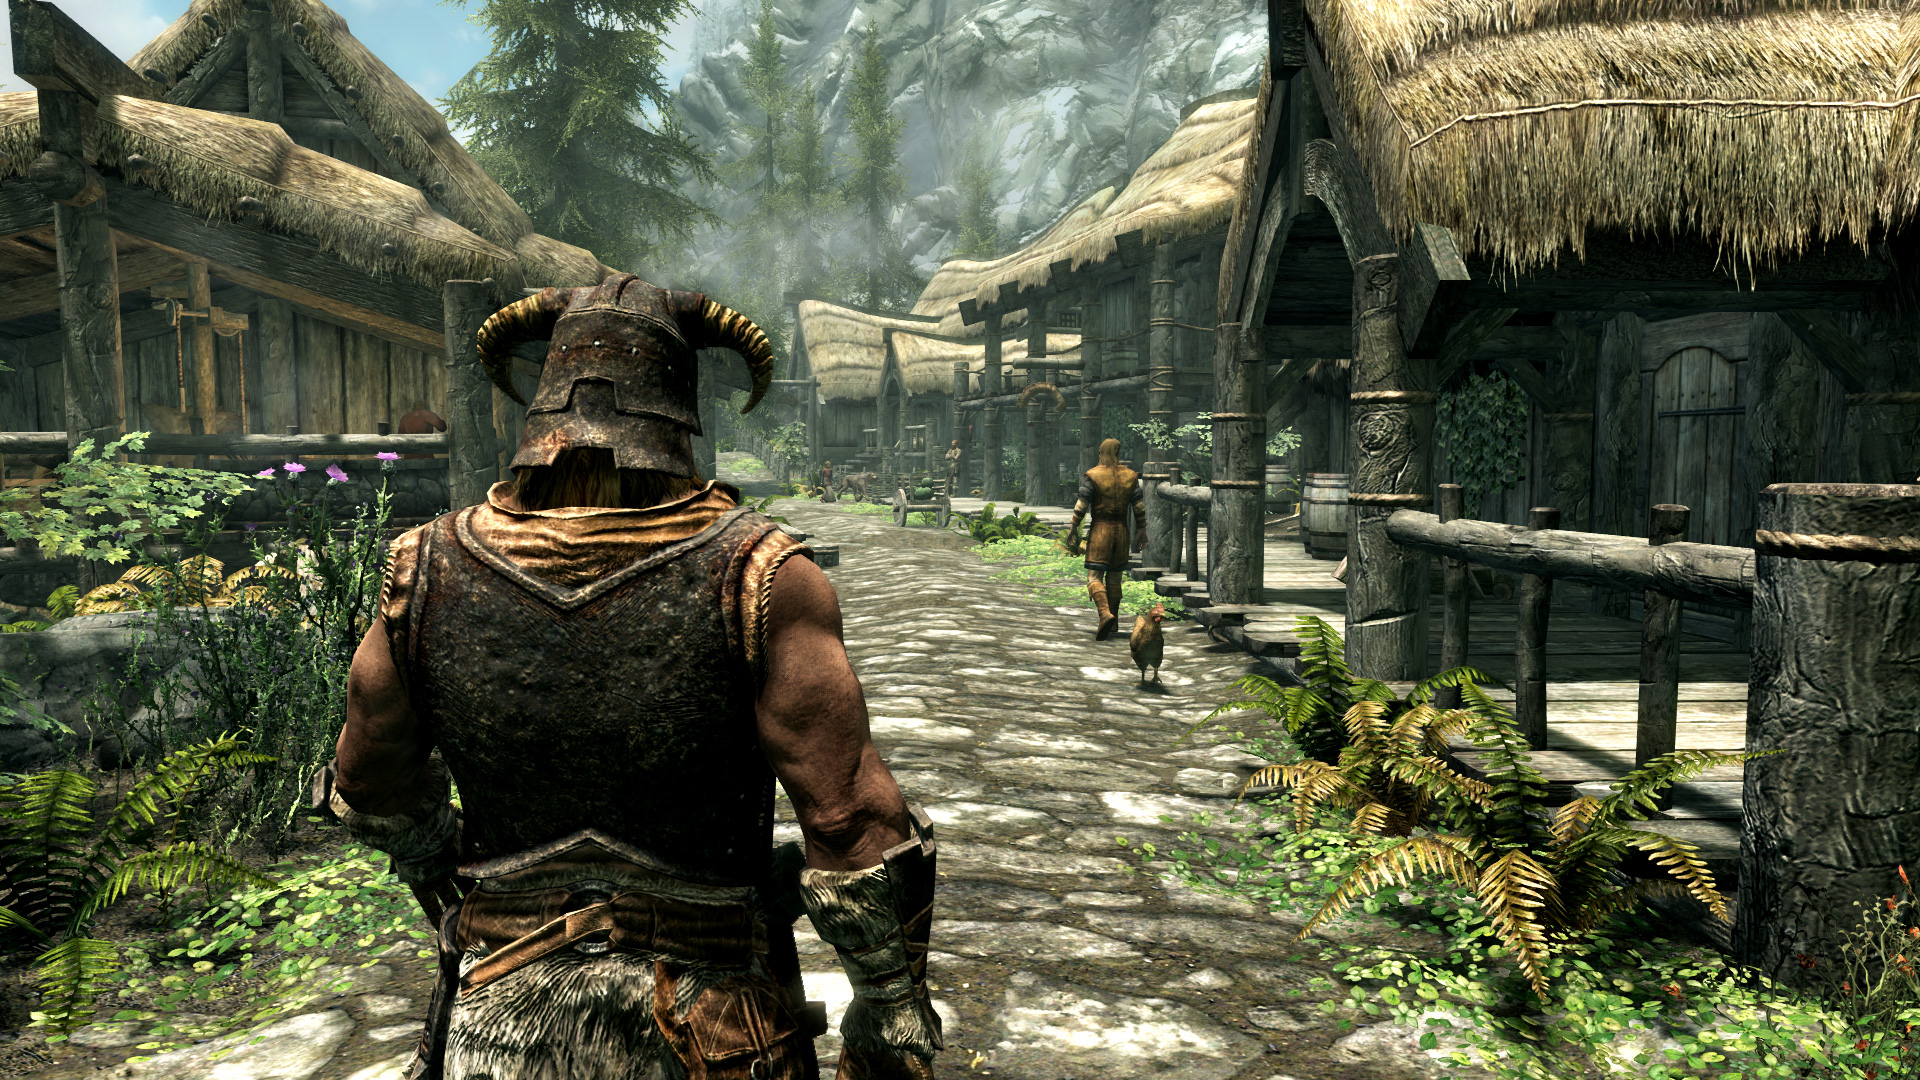
\includegraphics[width=0.7\textwidth]{experiments/uventura/AnaliseBibliometrica/Images/skyrim-remaster.jpg}
    \caption{Skyrim - 2011}
    \label{fig:uventura:bib-skyrim}
\end{figure}

\begin{figure}[H]
    \centering
    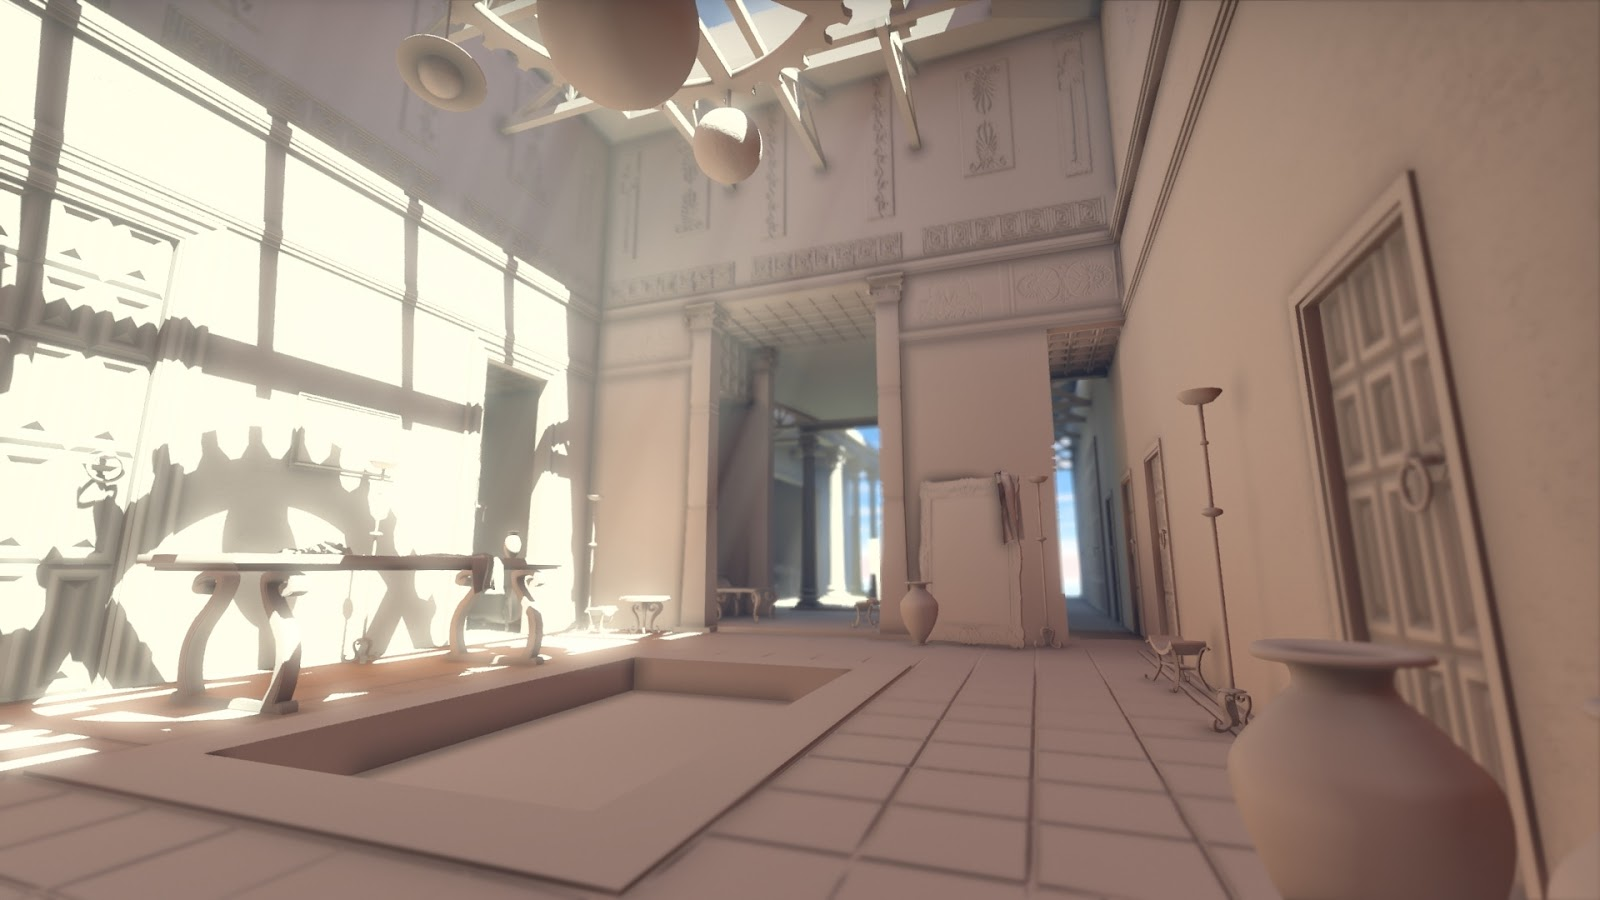
\includegraphics[width=0.7\textwidth]{experiments/uventura/AnaliseBibliometrica/Images/global-ilumination.jpg}
    \caption{Nvidia - Global Ilumination}
    \label{fig:uventura:bib-nvidia-global-ilumn}
\end{figure}

\subsection{Análise da Produção Mundial}

Em relação a produção intelectual dos artigos, é fundamental a compreensão dos seus produtores, assim, em relação aos países obtemos que sua relação é obtida graficamente como:

\begin{figure}[H]
    \centering
    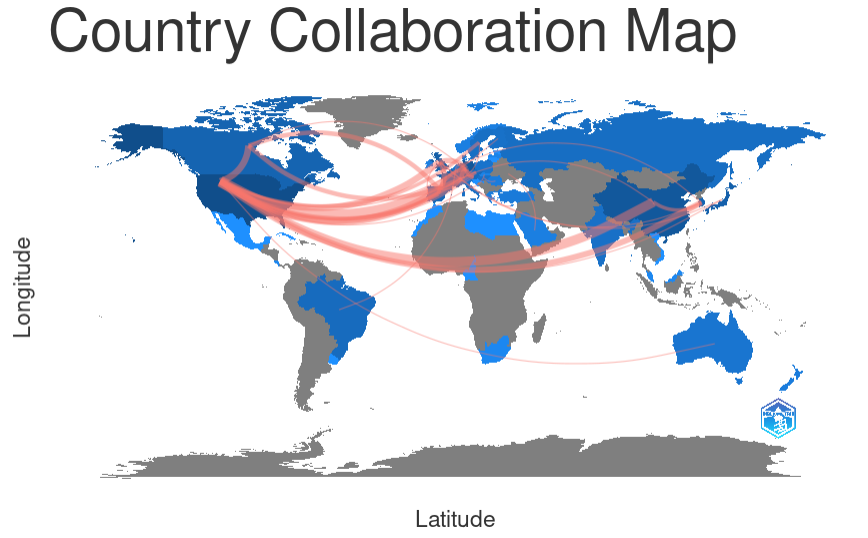
\includegraphics[width=0.8\textwidth]{experiments/uventura/AnaliseBibliometrica/Images/ColaboraçãoDePaíses.png}
    \caption{Colaboração Mundial}
    \label{fig:uventura:bib-country-colab}
\end{figure}

É importante observar que a relação entre Estados Unidos e Alemanha representa a em maior quantidade e apesar de não estar em evidência, o Brasil também é parte dos colaboradores mundiais.

Para maiores detalhes, temos então que os países que graficamente os 20 países que mais produzem em relação ao seus autores será:

\begin{figure}[H]
    \centering
    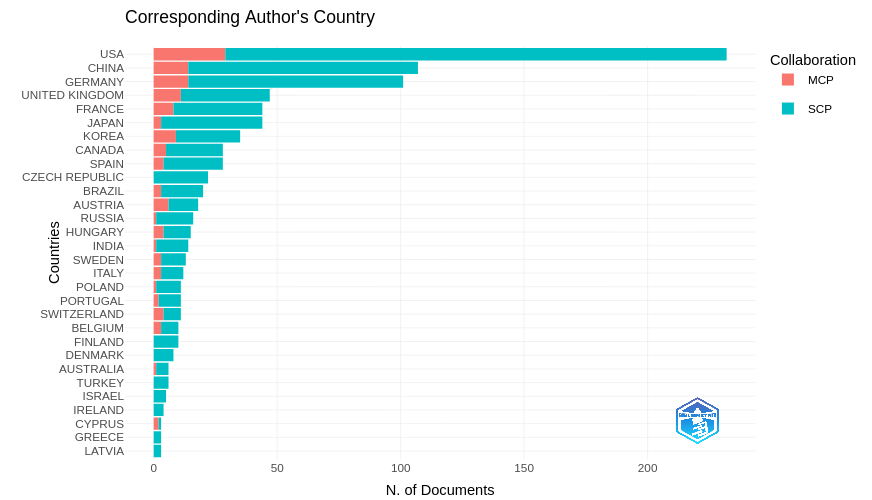
\includegraphics[width=0.8\textwidth]{experiments/uventura/AnaliseBibliometrica/Images/Corresponding Author's Country.png}
    \caption{Países com Maior Produção em Relação a Autores}
    \label{fig:uventura:bib-country-product}
\end{figure}

Portanto, é possível observar que Estados Unidos, China e Alemanha são aqueles com maior produção mundial, contudo, os Estados Unidos produz mais do que o dobro da China.


\section{Conclusão}

Diversos outros aspectos podem ser analisados além dos descritos, todavia, o objetivo tratava-se de analisar a produção em relação ao tópico, muito deve-se desenvolver considerando que é uma área que apenas nos últimos 20 anos pode crescer, anteriormente não haviam muitas oportunidades. Outras aplicações mais recentes têm surgido, uma delas é em casos como realidade virtual, que recentemente tem ganhado espaço e também está em crescimento.